%%%%%%%%%%%%%%%%%%%%%%%%%%%%%%%%%%%%%%%%%%%%%%%%%%%%%%%%%%%%%%%%%%%%%%
%%                     Not
%%%%%%%%%%%%%%%%%%%%%%%%%%%%%%%%%%%%%%%%%%%%%%%%%%%%%%%%%%%%%%%%%%%%%%
%\color{blue}
\subsection{Glyph: \glyph{Not}}\label{sec:not}

\begin{description}
 \item[SBO]\mbox{}\\ SBO:0000238 ! not.
 \item[origin]\mbox{}\\ One EPN (section~\ref{sec:EPNs}) or logical operator (section~\ref{sec:logic}).
 \item[target]\mbox{}\\  One modulation (section~\ref{sec:modulation}), stimulation (section~\ref{sec:stimulation}), catalysis (section~\ref{sec:catalysis}), inhibition (section~\ref{sec:inhibition}) or trigger (section~\ref{sec:trigger}) arcs.
 \item[node]\mbox{}\\ \glyph{not} is represented by a circle carrying the word ``not''.
 \end{description}

\begin{figure}[H]
  \centering
  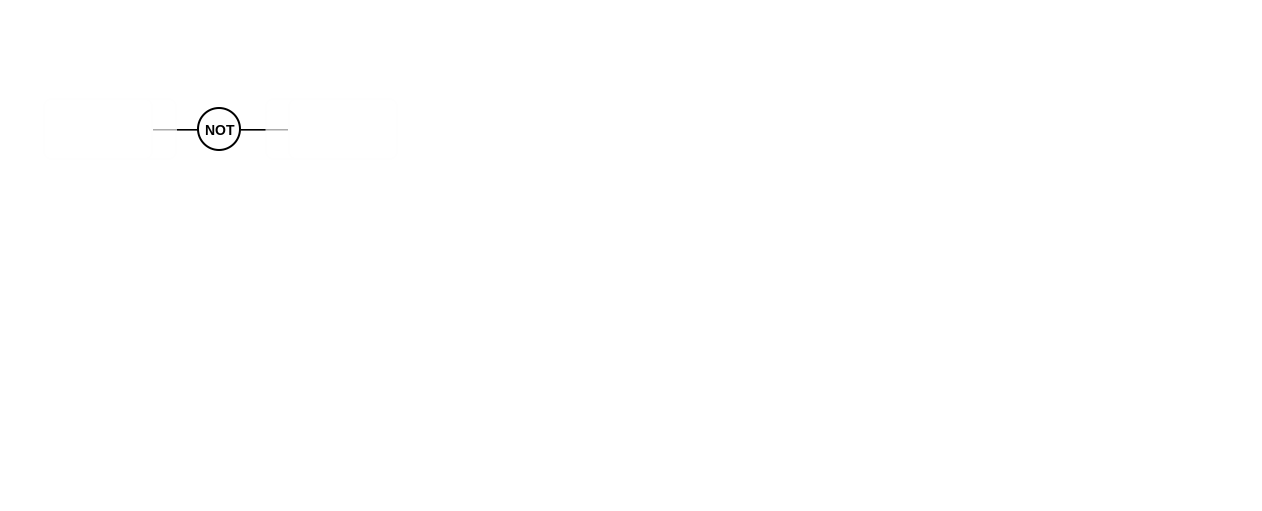
\includegraphics[scale = 0.5]{images/not}
  \caption{The \PD glyph for \glyph{not}.}
  \label{fig:not}
\end{figure}

